\section{memory.h File Reference}
\label{memory_8h}\index{memory.h@{memory.h}}
{\tt \#include $<$stdio.h$>$}\par
{\tt \#include \char`\"{}host.h\char`\"{}}\par
{\tt \#include \char`\"{}misc.h\char`\"{}}\par
{\tt \#include \char`\"{}machine.h\char`\"{}}\par
{\tt \#include \char`\"{}options.h\char`\"{}}\par
{\tt \#include \char`\"{}stats.h\char`\"{}}\par


Include dependency graph for memory.h:\nopagebreak
\begin{figure}[H]
\begin{center}
\leavevmode
\includegraphics[width=420pt]{memory_8h__incl}
\end{center}
\end{figure}


This graph shows which files directly or indirectly include this file:\nopagebreak
\begin{figure}[H]
\begin{center}
\leavevmode
\includegraphics[width=420pt]{memory_8h__dep__incl}
\end{center}
\end{figure}
\subsection*{Classes}
\begin{CompactItemize}
\item 
struct {\bf mem\_\-pte\_\-t}
\item 
struct {\bf mem\_\-page\_\-link\_\-t}
\item 
struct {\bf mem\_\-t}
\end{CompactItemize}
\subsection*{Defines}
\begin{CompactItemize}
\item 
\#define {\bf MEM\_\-PTAB\_\-SIZE}~(256$\ast$1024)
\item 
\#define {\bf MEM\_\-LOG\_\-PTAB\_\-SIZE}~18
\item 
\#define {\bf MAX\_\-LEV}~3
\item 
\#define {\bf PAGE\_\-SIZE}~4096
\item 
\#define {\bf PAGE\_\-SHIFT}~12
\item 
\#define {\bf PAGE\_\-TABLE\_\-ADDR}(T, A)~((((((A)$>$$>$PAGE\_\-SHIFT)$<$$<$4)+(T)) + 0x00080000) \& 0x03ffffff)
\item 
\#define {\bf DO\_\-NOT\_\-TRANSLATE}~(-1)
\item 
\#define {\bf MEM\_\-PTAB\_\-SET}(ADDR)~(((ADDR) $>$$>$ MD\_\-LOG\_\-PAGE\_\-SIZE) \& (MEM\_\-PTAB\_\-SIZE - 1))
\item 
\#define {\bf MEM\_\-PTAB\_\-TAG}(ADDR)~((ADDR) $>$$>$ (MD\_\-LOG\_\-PAGE\_\-SIZE + MEM\_\-LOG\_\-PTAB\_\-SIZE))
\item 
\#define {\bf MEM\_\-PTE\_\-ADDR}(PTE, IDX)
\item 
\#define {\bf MEM\_\-PAGE}(MEM, ADDR, DIRTY)~mem\_\-translate((MEM), (ADDR), (DIRTY))
\item 
\#define {\bf MEM\_\-OFFSET}(ADDR)~((ADDR) \& (MD\_\-PAGE\_\-SIZE - 1))
\item 
\#define {\bf MEM\_\-ADDR2HOST}(MEM, ADDR)~MEM\_\-PAGE(MEM, ADDR, 0)+MEM\_\-OFFSET(ADDR)
\item 
\#define {\bf MEM\_\-TICKLE}(MEM, ADDR)
\item 
\#define {\bf MEM\_\-FORALL}(MEM, ITER, PTE)
\item 
\#define {\bf MEM\_\-READ}(MEM, ADDR, TYPE)
\item 
\#define {\bf MEM\_\-WRITE}(MEM, ADDR, TYPE, VAL)
\item 
\#define {\bf MEM\_\-READ\_\-BYTE}(MEM, ADDR)~MEM\_\-READ(MEM, ADDR, {\bf byte\_\-t})
\item 
\#define {\bf MEM\_\-READ\_\-SBYTE}(MEM, ADDR)~MEM\_\-READ(MEM, ADDR, {\bf sbyte\_\-t})
\item 
\#define {\bf MEM\_\-READ\_\-WORD}(MEM, ADDR)~MD\_\-SWAPW(MEM\_\-READ(MEM, ADDR, {\bf word\_\-t}))
\item 
\#define {\bf MEM\_\-READ\_\-SWORD}(MEM, ADDR)~MD\_\-SWAPW(MEM\_\-READ(MEM, ADDR, {\bf sword\_\-t}))
\item 
\#define {\bf MEM\_\-READ\_\-DWORD}(MEM, ADDR)~MD\_\-SWAPD(MEM\_\-READ(MEM, ADDR, {\bf dword\_\-t}))
\item 
\#define {\bf MEM\_\-READ\_\-SDWORD}(MEM, ADDR)~MD\_\-SWAPD(MEM\_\-READ(MEM, ADDR, {\bf sdword\_\-t}))
\item 
\#define {\bf MEM\_\-WRITE\_\-BYTE}(MEM, ADDR, VAL)~MEM\_\-WRITE(MEM, ADDR, {\bf byte\_\-t}, VAL)
\item 
\#define {\bf MEM\_\-WRITE\_\-SBYTE}(MEM, ADDR, VAL)~MEM\_\-WRITE(MEM, ADDR, {\bf sbyte\_\-t}, VAL)
\item 
\#define {\bf MEM\_\-WRITE\_\-WORD}(MEM, ADDR, VAL)~MEM\_\-WRITE(MEM, ADDR, {\bf word\_\-t}, MD\_\-SWAPW(VAL));
\item 
\#define {\bf MEM\_\-WRITE\_\-SWORD}(MEM, ADDR, VAL)~MEM\_\-WRITE(MEM, ADDR, {\bf sword\_\-t}, MD\_\-SWAPW(VAL));
\item 
\#define {\bf MEM\_\-WRITE\_\-DWORD}(MEM, ADDR, VAL)~MEM\_\-WRITE(MEM, ADDR, {\bf dword\_\-t}, MD\_\-SWAPD(VAL));
\item 
\#define {\bf MEM\_\-WRITE\_\-SDWORD}(MEM, ADDR, VAL)~MEM\_\-WRITE(MEM, ADDR, {\bf sdword\_\-t}, MD\_\-SWAPD(VAL));
\item 
\#define {\bf MEM\_\-WRITE\_\-SFLOAT}(MEM, ADDR, VAL)~MEM\_\-WRITE(MEM, ADDR, {\bf sfloat\_\-t}, MD\_\-SWAPD(VAL));
\item 
\#define {\bf MEM\_\-WRITE\_\-DFLOAT}(MEM, ADDR, VAL)~MEM\_\-WRITE(MEM, ADDR, {\bf dfloat\_\-t}, MD\_\-SWAPQ(VAL));
\end{CompactItemize}
\subsection*{Enumerations}
\begin{CompactItemize}
\item 
enum {\bf mem\_\-cmd} \{ {\bf Read}, 
{\bf Write}
 \}
\end{CompactItemize}
\subsection*{Functions}
\begin{CompactItemize}
\item 
struct {\bf mem\_\-t} $\ast$ {\bf mem\_\-create} (char $\ast$name)
\item 
{\bf byte\_\-t} $\ast$ {\bf mem\_\-translate} (struct {\bf mem\_\-t} $\ast$mem, {\bf md\_\-addr\_\-t} addr, int dirty)
\item 
void {\bf mem\_\-newpage} (struct {\bf mem\_\-t} $\ast$mem, {\bf md\_\-addr\_\-t} addr)
\item 
void {\bf wipe\_\-memory} (struct {\bf mem\_\-t} $\ast$mem)
\item 
{\bf md\_\-addr\_\-t} {\bf mem\_\-newmap} (struct {\bf mem\_\-t} $\ast$mem, {\bf md\_\-addr\_\-t} addr, size\_\-t length, int mmap)
\item 
{\bf md\_\-addr\_\-t} {\bf mem\_\-newmap2} (struct {\bf mem\_\-t} $\ast$mem, {\bf md\_\-addr\_\-t} addr, {\bf md\_\-addr\_\-t} our\_\-addr, size\_\-t length, int mmap)
\item 
void {\bf mem\_\-delmap} (struct {\bf mem\_\-t} $\ast$mem, {\bf md\_\-addr\_\-t} addr, size\_\-t length)
\item 
enum {\bf md\_\-fault\_\-type} {\bf mem\_\-check\_\-fault} (struct {\bf mem\_\-t} $\ast$mem, enum {\bf mem\_\-cmd} cmd, {\bf md\_\-addr\_\-t} addr, int nbytes)
\item 
enum {\bf md\_\-fault\_\-type} {\bf mem\_\-access} (int core\_\-id, struct {\bf mem\_\-t} $\ast$mem, enum {\bf mem\_\-cmd} cmd, {\bf md\_\-addr\_\-t} addr, void $\ast$vp, int nbytes)
\item 
void {\bf mem\_\-reg\_\-stats} (struct {\bf mem\_\-t} $\ast$mem, struct {\bf stat\_\-sdb\_\-t} $\ast$sdb)
\item 
void {\bf mem\_\-init} (struct {\bf mem\_\-t} $\ast$mem)
\item 
enum {\bf md\_\-fault\_\-type} {\bf mem\_\-strcpy} (int core\_\-id, {\bf mem\_\-access\_\-fn} mem\_\-fn, struct {\bf mem\_\-t} $\ast$mem, enum {\bf mem\_\-cmd} cmd, {\bf md\_\-addr\_\-t} addr, char $\ast${\bf s})
\item 
enum {\bf md\_\-fault\_\-type} {\bf mem\_\-bcopy} (int core\_\-id, {\bf mem\_\-access\_\-fn} mem\_\-fn, struct {\bf mem\_\-t} $\ast$mem, enum {\bf mem\_\-cmd} cmd, {\bf md\_\-addr\_\-t} addr, void $\ast$vp, int nbytes)
\item 
{\bf md\_\-paddr\_\-t} {\bf v2p\_\-translate} (int core\_\-id, {\bf md\_\-addr\_\-t} virt\_\-addr)
\item 
int {\bf page\_\-owner} ({\bf md\_\-paddr\_\-t} paddr)
\end{CompactItemize}
\subsection*{Variables}
\begin{CompactItemize}
\item 
enum {\bf md\_\-fault\_\-type}($\ast$ {\bf mem\_\-access\_\-fn} )(int core\_\-id, struct {\bf mem\_\-t} $\ast$mem, enum {\bf mem\_\-cmd} cmd, {\bf md\_\-addr\_\-t} addr, void $\ast$p, int nbytes)
\end{CompactItemize}


\subsection{Define Documentation}
\index{memory.h@{memory.h}!DO\_\-NOT\_\-TRANSLATE@{DO\_\-NOT\_\-TRANSLATE}}
\index{DO\_\-NOT\_\-TRANSLATE@{DO\_\-NOT\_\-TRANSLATE}!memory.h@{memory.h}}
\subsubsection[{DO\_\-NOT\_\-TRANSLATE}]{\setlength{\rightskip}{0pt plus 5cm}\#define DO\_\-NOT\_\-TRANSLATE~(-1)}\label{memory_8h_2d833799add0043705e93c62bd718532}




Definition at line 157 of file memory.h.

Referenced by cache\_\-enqueuable(), cache\_\-enqueuable\_\-llc(), cache\_\-enqueue(), cache\_\-enqueue\_\-llc(), cache\_\-prefetch(), cache\_\-prefetch\_\-llc(), and cache\_\-process().\index{memory.h@{memory.h}!MAX\_\-LEV@{MAX\_\-LEV}}
\index{MAX\_\-LEV@{MAX\_\-LEV}!memory.h@{memory.h}}
\subsubsection[{MAX\_\-LEV}]{\setlength{\rightskip}{0pt plus 5cm}\#define MAX\_\-LEV~3}\label{memory_8h_af900f23f86c82aca5502edba1f68fcf}




Definition at line 140 of file memory.h.\index{memory.h@{memory.h}!MEM\_\-ADDR2HOST@{MEM\_\-ADDR2HOST}}
\index{MEM\_\-ADDR2HOST@{MEM\_\-ADDR2HOST}!memory.h@{memory.h}}
\subsubsection[{MEM\_\-ADDR2HOST}]{\setlength{\rightskip}{0pt plus 5cm}\#define MEM\_\-ADDR2HOST(MEM, \/  ADDR)~MEM\_\-PAGE(MEM, ADDR, 0)+MEM\_\-OFFSET(ADDR)}\label{memory_8h_f451f14e7eb88fc1bd2df4da94391f29}




Definition at line 235 of file memory.h.\index{memory.h@{memory.h}!MEM\_\-FORALL@{MEM\_\-FORALL}}
\index{MEM\_\-FORALL@{MEM\_\-FORALL}!memory.h@{memory.h}}
\subsubsection[{MEM\_\-FORALL}]{\setlength{\rightskip}{0pt plus 5cm}\#define MEM\_\-FORALL(MEM, \/  ITER, \/  PTE)}\label{memory_8h_cd714378a3b9e45e84ab96a1a808fb0c}


\textbf{Value:}

\begin{Code}\begin{verbatim}for ((ITER)=0; (ITER) < MEM_PTAB_SIZE; (ITER)++)      \
    for ((PTE)=(MEM)->ptab[(ITER)]; (PTE) != NULL; (PTE)=(PTE)->next)
\end{verbatim}
\end{Code}


Definition at line 245 of file memory.h.\index{memory.h@{memory.h}!MEM\_\-LOG\_\-PTAB\_\-SIZE@{MEM\_\-LOG\_\-PTAB\_\-SIZE}}
\index{MEM\_\-LOG\_\-PTAB\_\-SIZE@{MEM\_\-LOG\_\-PTAB\_\-SIZE}!memory.h@{memory.h}}
\subsubsection[{MEM\_\-LOG\_\-PTAB\_\-SIZE}]{\setlength{\rightskip}{0pt plus 5cm}\#define MEM\_\-LOG\_\-PTAB\_\-SIZE~18}\label{memory_8h_4c16bab1d72c131bb7d22f499316fc29}




Definition at line 139 of file memory.h.\index{memory.h@{memory.h}!MEM\_\-OFFSET@{MEM\_\-OFFSET}}
\index{MEM\_\-OFFSET@{MEM\_\-OFFSET}!memory.h@{memory.h}}
\subsubsection[{MEM\_\-OFFSET}]{\setlength{\rightskip}{0pt plus 5cm}\#define MEM\_\-OFFSET(ADDR)~((ADDR) \& (MD\_\-PAGE\_\-SIZE - 1))}\label{memory_8h_fca35a65688a3a304cf8628ccc320aa2}




Definition at line 233 of file memory.h.\index{memory.h@{memory.h}!MEM\_\-PAGE@{MEM\_\-PAGE}}
\index{MEM\_\-PAGE@{MEM\_\-PAGE}!memory.h@{memory.h}}
\subsubsection[{MEM\_\-PAGE}]{\setlength{\rightskip}{0pt plus 5cm}\#define MEM\_\-PAGE(MEM, \/  ADDR, \/  DIRTY)~mem\_\-translate((MEM), (ADDR), (DIRTY))}\label{memory_8h_16fb3c34501493d993b7e4ff81e83099}




Definition at line 230 of file memory.h.\index{memory.h@{memory.h}!MEM\_\-PTAB\_\-SET@{MEM\_\-PTAB\_\-SET}}
\index{MEM\_\-PTAB\_\-SET@{MEM\_\-PTAB\_\-SET}!memory.h@{memory.h}}
\subsubsection[{MEM\_\-PTAB\_\-SET}]{\setlength{\rightskip}{0pt plus 5cm}\#define MEM\_\-PTAB\_\-SET(ADDR)~(((ADDR) $>$$>$ MD\_\-LOG\_\-PAGE\_\-SIZE) \& (MEM\_\-PTAB\_\-SIZE - 1))}\label{memory_8h_4ab2e3db8a6c800c8b61d638bab14a97}




Definition at line 217 of file memory.h.\index{memory.h@{memory.h}!MEM\_\-PTAB\_\-SIZE@{MEM\_\-PTAB\_\-SIZE}}
\index{MEM\_\-PTAB\_\-SIZE@{MEM\_\-PTAB\_\-SIZE}!memory.h@{memory.h}}
\subsubsection[{MEM\_\-PTAB\_\-SIZE}]{\setlength{\rightskip}{0pt plus 5cm}\#define MEM\_\-PTAB\_\-SIZE~(256$\ast$1024)}\label{memory_8h_5b1198a1e1df589729b1f3533005ae3e}




Definition at line 138 of file memory.h.\index{memory.h@{memory.h}!MEM\_\-PTAB\_\-TAG@{MEM\_\-PTAB\_\-TAG}}
\index{MEM\_\-PTAB\_\-TAG@{MEM\_\-PTAB\_\-TAG}!memory.h@{memory.h}}
\subsubsection[{MEM\_\-PTAB\_\-TAG}]{\setlength{\rightskip}{0pt plus 5cm}\#define MEM\_\-PTAB\_\-TAG(ADDR)~((ADDR) $>$$>$ (MD\_\-LOG\_\-PAGE\_\-SIZE + MEM\_\-LOG\_\-PTAB\_\-SIZE))}\label{memory_8h_22dca2aefeec3059d2f9799d085a024c}




Definition at line 221 of file memory.h.\index{memory.h@{memory.h}!MEM\_\-PTE\_\-ADDR@{MEM\_\-PTE\_\-ADDR}}
\index{MEM\_\-PTE\_\-ADDR@{MEM\_\-PTE\_\-ADDR}!memory.h@{memory.h}}
\subsubsection[{MEM\_\-PTE\_\-ADDR}]{\setlength{\rightskip}{0pt plus 5cm}\#define MEM\_\-PTE\_\-ADDR(PTE, \/  IDX)}\label{memory_8h_5181baa328a8761b4e4664e290eb2911}


\textbf{Value:}

\begin{Code}\begin{verbatim}(((PTE)->tag << (MD_LOG_PAGE_SIZE + MEM_LOG_PTAB_SIZE))    \
   | ((IDX) << MD_LOG_PAGE_SIZE))
\end{verbatim}
\end{Code}


Definition at line 225 of file memory.h.\index{memory.h@{memory.h}!MEM\_\-READ@{MEM\_\-READ}}
\index{MEM\_\-READ@{MEM\_\-READ}!memory.h@{memory.h}}
\subsubsection[{MEM\_\-READ}]{\setlength{\rightskip}{0pt plus 5cm}\#define MEM\_\-READ(MEM, \/  ADDR, \/  TYPE)}\label{memory_8h_ade0bb90ecee3019c4ed93501d7d3603}


\textbf{Value:}

\begin{Code}\begin{verbatim}(MEM_PAGE(MEM, (md_addr_t)(ADDR),0)          \
   ? *((TYPE *)(MEM_PAGE(MEM, (md_addr_t)(ADDR),0) + MEM_OFFSET(ADDR)))  \
   : /* page not yet allocated, return zero value */ 0)
\end{verbatim}
\end{Code}


Definition at line 274 of file memory.h.\index{memory.h@{memory.h}!MEM\_\-READ\_\-BYTE@{MEM\_\-READ\_\-BYTE}}
\index{MEM\_\-READ\_\-BYTE@{MEM\_\-READ\_\-BYTE}!memory.h@{memory.h}}
\subsubsection[{MEM\_\-READ\_\-BYTE}]{\setlength{\rightskip}{0pt plus 5cm}\#define MEM\_\-READ\_\-BYTE(MEM, \/  ADDR)~MEM\_\-READ(MEM, ADDR, {\bf byte\_\-t})}\label{memory_8h_85d685b6654896c2141a548a2d891f1e}




Definition at line 287 of file memory.h.\index{memory.h@{memory.h}!MEM\_\-READ\_\-DWORD@{MEM\_\-READ\_\-DWORD}}
\index{MEM\_\-READ\_\-DWORD@{MEM\_\-READ\_\-DWORD}!memory.h@{memory.h}}
\subsubsection[{MEM\_\-READ\_\-DWORD}]{\setlength{\rightskip}{0pt plus 5cm}\#define MEM\_\-READ\_\-DWORD(MEM, \/  ADDR)~MD\_\-SWAPD(MEM\_\-READ(MEM, ADDR, {\bf dword\_\-t}))}\label{memory_8h_5c05e229b73207dac15220b595774e64}




Definition at line 291 of file memory.h.\index{memory.h@{memory.h}!MEM\_\-READ\_\-SBYTE@{MEM\_\-READ\_\-SBYTE}}
\index{MEM\_\-READ\_\-SBYTE@{MEM\_\-READ\_\-SBYTE}!memory.h@{memory.h}}
\subsubsection[{MEM\_\-READ\_\-SBYTE}]{\setlength{\rightskip}{0pt plus 5cm}\#define MEM\_\-READ\_\-SBYTE(MEM, \/  ADDR)~MEM\_\-READ(MEM, ADDR, {\bf sbyte\_\-t})}\label{memory_8h_c766bf126503da78f89f84b336b45235}




Definition at line 288 of file memory.h.\index{memory.h@{memory.h}!MEM\_\-READ\_\-SDWORD@{MEM\_\-READ\_\-SDWORD}}
\index{MEM\_\-READ\_\-SDWORD@{MEM\_\-READ\_\-SDWORD}!memory.h@{memory.h}}
\subsubsection[{MEM\_\-READ\_\-SDWORD}]{\setlength{\rightskip}{0pt plus 5cm}\#define MEM\_\-READ\_\-SDWORD(MEM, \/  ADDR)~MD\_\-SWAPD(MEM\_\-READ(MEM, ADDR, {\bf sdword\_\-t}))}\label{memory_8h_2990be943ca21b53b026d1ef6e0f2e90}




Definition at line 292 of file memory.h.\index{memory.h@{memory.h}!MEM\_\-READ\_\-SWORD@{MEM\_\-READ\_\-SWORD}}
\index{MEM\_\-READ\_\-SWORD@{MEM\_\-READ\_\-SWORD}!memory.h@{memory.h}}
\subsubsection[{MEM\_\-READ\_\-SWORD}]{\setlength{\rightskip}{0pt plus 5cm}\#define MEM\_\-READ\_\-SWORD(MEM, \/  ADDR)~MD\_\-SWAPW(MEM\_\-READ(MEM, ADDR, {\bf sword\_\-t}))}\label{memory_8h_327b962e79529d0acb86308d0b0c7fd7}




Definition at line 290 of file memory.h.\index{memory.h@{memory.h}!MEM\_\-READ\_\-WORD@{MEM\_\-READ\_\-WORD}}
\index{MEM\_\-READ\_\-WORD@{MEM\_\-READ\_\-WORD}!memory.h@{memory.h}}
\subsubsection[{MEM\_\-READ\_\-WORD}]{\setlength{\rightskip}{0pt plus 5cm}\#define MEM\_\-READ\_\-WORD(MEM, \/  ADDR)~MD\_\-SWAPW(MEM\_\-READ(MEM, ADDR, {\bf word\_\-t}))}\label{memory_8h_df7ec3c2beb389755a2368fcdb4d3c1d}




Definition at line 289 of file memory.h.\index{memory.h@{memory.h}!MEM\_\-TICKLE@{MEM\_\-TICKLE}}
\index{MEM\_\-TICKLE@{MEM\_\-TICKLE}!memory.h@{memory.h}}
\subsubsection[{MEM\_\-TICKLE}]{\setlength{\rightskip}{0pt plus 5cm}\#define MEM\_\-TICKLE(MEM, \/  ADDR)}\label{memory_8h_192d28cbc253d5a267f35375ffb19fb9}


\textbf{Value:}

\begin{Code}\begin{verbatim}((!MEM_PAGE(MEM, ADDR, 0)            \
    ? (/* allocate page at address ADDR */        \
      mem_newpage(MEM, ADDR))            \
    : (/* nada... */ (void)0)))
\end{verbatim}
\end{Code}


Definition at line 238 of file memory.h.\index{memory.h@{memory.h}!MEM\_\-WRITE@{MEM\_\-WRITE}}
\index{MEM\_\-WRITE@{MEM\_\-WRITE}!memory.h@{memory.h}}
\subsubsection[{MEM\_\-WRITE}]{\setlength{\rightskip}{0pt plus 5cm}\#define MEM\_\-WRITE(MEM, \/  ADDR, \/  TYPE, \/  VAL)}\label{memory_8h_28259663d5e1ed1f30217b2de915f049}


\textbf{Value:}

\begin{Code}\begin{verbatim}(MEM_TICKLE(MEM, (md_addr_t)(ADDR)),          \
   *((TYPE *)(MEM_PAGE(MEM, (md_addr_t)(ADDR),1) + MEM_OFFSET(ADDR))) = (VAL))
\end{verbatim}
\end{Code}


Definition at line 281 of file memory.h.\index{memory.h@{memory.h}!MEM\_\-WRITE\_\-BYTE@{MEM\_\-WRITE\_\-BYTE}}
\index{MEM\_\-WRITE\_\-BYTE@{MEM\_\-WRITE\_\-BYTE}!memory.h@{memory.h}}
\subsubsection[{MEM\_\-WRITE\_\-BYTE}]{\setlength{\rightskip}{0pt plus 5cm}\#define MEM\_\-WRITE\_\-BYTE(MEM, \/  ADDR, \/  VAL)~MEM\_\-WRITE(MEM, ADDR, {\bf byte\_\-t}, VAL)}\label{memory_8h_724551f165f8e43838a01246e76ad4e8}




Definition at line 305 of file memory.h.\index{memory.h@{memory.h}!MEM\_\-WRITE\_\-DFLOAT@{MEM\_\-WRITE\_\-DFLOAT}}
\index{MEM\_\-WRITE\_\-DFLOAT@{MEM\_\-WRITE\_\-DFLOAT}!memory.h@{memory.h}}
\subsubsection[{MEM\_\-WRITE\_\-DFLOAT}]{\setlength{\rightskip}{0pt plus 5cm}\#define MEM\_\-WRITE\_\-DFLOAT(MEM, \/  ADDR, \/  VAL)~MEM\_\-WRITE(MEM, ADDR, {\bf dfloat\_\-t}, MD\_\-SWAPQ(VAL));}\label{memory_8h_e2ed34009527ba3d439904f887e3484d}




Definition at line 312 of file memory.h.\index{memory.h@{memory.h}!MEM\_\-WRITE\_\-DWORD@{MEM\_\-WRITE\_\-DWORD}}
\index{MEM\_\-WRITE\_\-DWORD@{MEM\_\-WRITE\_\-DWORD}!memory.h@{memory.h}}
\subsubsection[{MEM\_\-WRITE\_\-DWORD}]{\setlength{\rightskip}{0pt plus 5cm}\#define MEM\_\-WRITE\_\-DWORD(MEM, \/  ADDR, \/  VAL)~MEM\_\-WRITE(MEM, ADDR, {\bf dword\_\-t}, MD\_\-SWAPD(VAL));}\label{memory_8h_f75c0d05b5dc2ccbdf46593904b332aa}




Definition at line 309 of file memory.h.\index{memory.h@{memory.h}!MEM\_\-WRITE\_\-SBYTE@{MEM\_\-WRITE\_\-SBYTE}}
\index{MEM\_\-WRITE\_\-SBYTE@{MEM\_\-WRITE\_\-SBYTE}!memory.h@{memory.h}}
\subsubsection[{MEM\_\-WRITE\_\-SBYTE}]{\setlength{\rightskip}{0pt plus 5cm}\#define MEM\_\-WRITE\_\-SBYTE(MEM, \/  ADDR, \/  VAL)~MEM\_\-WRITE(MEM, ADDR, {\bf sbyte\_\-t}, VAL)}\label{memory_8h_8ee284de1eb9b6f435752a3a17eb9755}




Definition at line 306 of file memory.h.\index{memory.h@{memory.h}!MEM\_\-WRITE\_\-SDWORD@{MEM\_\-WRITE\_\-SDWORD}}
\index{MEM\_\-WRITE\_\-SDWORD@{MEM\_\-WRITE\_\-SDWORD}!memory.h@{memory.h}}
\subsubsection[{MEM\_\-WRITE\_\-SDWORD}]{\setlength{\rightskip}{0pt plus 5cm}\#define MEM\_\-WRITE\_\-SDWORD(MEM, \/  ADDR, \/  VAL)~MEM\_\-WRITE(MEM, ADDR, {\bf sdword\_\-t}, MD\_\-SWAPD(VAL));}\label{memory_8h_ada0fda16a4e39b7f4f4e8057ab87f9f}




Definition at line 310 of file memory.h.\index{memory.h@{memory.h}!MEM\_\-WRITE\_\-SFLOAT@{MEM\_\-WRITE\_\-SFLOAT}}
\index{MEM\_\-WRITE\_\-SFLOAT@{MEM\_\-WRITE\_\-SFLOAT}!memory.h@{memory.h}}
\subsubsection[{MEM\_\-WRITE\_\-SFLOAT}]{\setlength{\rightskip}{0pt plus 5cm}\#define MEM\_\-WRITE\_\-SFLOAT(MEM, \/  ADDR, \/  VAL)~MEM\_\-WRITE(MEM, ADDR, {\bf sfloat\_\-t}, MD\_\-SWAPD(VAL));}\label{memory_8h_b4d509a26e8c65c9e57c97a924b74156}




Definition at line 311 of file memory.h.\index{memory.h@{memory.h}!MEM\_\-WRITE\_\-SWORD@{MEM\_\-WRITE\_\-SWORD}}
\index{MEM\_\-WRITE\_\-SWORD@{MEM\_\-WRITE\_\-SWORD}!memory.h@{memory.h}}
\subsubsection[{MEM\_\-WRITE\_\-SWORD}]{\setlength{\rightskip}{0pt plus 5cm}\#define MEM\_\-WRITE\_\-SWORD(MEM, \/  ADDR, \/  VAL)~MEM\_\-WRITE(MEM, ADDR, {\bf sword\_\-t}, MD\_\-SWAPW(VAL));}\label{memory_8h_1aa3f5f5b1649e050852f0d58d5f3256}




Definition at line 308 of file memory.h.\index{memory.h@{memory.h}!MEM\_\-WRITE\_\-WORD@{MEM\_\-WRITE\_\-WORD}}
\index{MEM\_\-WRITE\_\-WORD@{MEM\_\-WRITE\_\-WORD}!memory.h@{memory.h}}
\subsubsection[{MEM\_\-WRITE\_\-WORD}]{\setlength{\rightskip}{0pt plus 5cm}\#define MEM\_\-WRITE\_\-WORD(MEM, \/  ADDR, \/  VAL)~MEM\_\-WRITE(MEM, ADDR, {\bf word\_\-t}, MD\_\-SWAPW(VAL));}\label{memory_8h_f73ab32adca03428d5ff21ea43d9f473}




Definition at line 307 of file memory.h.\index{memory.h@{memory.h}!PAGE\_\-SHIFT@{PAGE\_\-SHIFT}}
\index{PAGE\_\-SHIFT@{PAGE\_\-SHIFT}!memory.h@{memory.h}}
\subsubsection[{PAGE\_\-SHIFT}]{\setlength{\rightskip}{0pt plus 5cm}\#define PAGE\_\-SHIFT~12}\label{memory_8h_850d80ca2291d26b40dc6b25c419f81a}




Definition at line 145 of file memory.h.

Referenced by core\_\-fetch\_\-STM\_\-t::step(), and core\_\-fetch\_\-DPM\_\-t::step().\index{memory.h@{memory.h}!PAGE\_\-SIZE@{PAGE\_\-SIZE}}
\index{PAGE\_\-SIZE@{PAGE\_\-SIZE}!memory.h@{memory.h}}
\subsubsection[{PAGE\_\-SIZE}]{\setlength{\rightskip}{0pt plus 5cm}\#define PAGE\_\-SIZE~4096}\label{memory_8h_7d467c1d283fdfa1f2081ba1e0d01b6e}




Definition at line 144 of file memory.h.

Referenced by cache\_\-process(), and cache\_\-process\_\-llc().\index{memory.h@{memory.h}!PAGE\_\-TABLE\_\-ADDR@{PAGE\_\-TABLE\_\-ADDR}}
\index{PAGE\_\-TABLE\_\-ADDR@{PAGE\_\-TABLE\_\-ADDR}!memory.h@{memory.h}}
\subsubsection[{PAGE\_\-TABLE\_\-ADDR}]{\setlength{\rightskip}{0pt plus 5cm}\#define PAGE\_\-TABLE\_\-ADDR(T, \/  A)~((((((A)$>$$>$PAGE\_\-SHIFT)$<$$<$4)+(T)) + 0x00080000) \& 0x03ffffff)}\label{memory_8h_628a3729ebbf0306b93db41d9b34b0ca}




Definition at line 156 of file memory.h.

Referenced by core\_\-exec\_\-STM\_\-t::LDQ\_\-schedule(), core\_\-exec\_\-DPM\_\-t::LDQ\_\-schedule(), sim\_\-fastfwd(), core\_\-fetch\_\-STM\_\-t::step(), core\_\-fetch\_\-DPM\_\-t::step(), core\_\-exec\_\-STM\_\-t::STQ\_\-deallocate\_\-std(), and core\_\-exec\_\-DPM\_\-t::STQ\_\-deallocate\_\-std().

\subsection{Enumeration Type Documentation}
\index{memory.h@{memory.h}!mem\_\-cmd@{mem\_\-cmd}}
\index{mem\_\-cmd@{mem\_\-cmd}!memory.h@{memory.h}}
\subsubsection[{mem\_\-cmd}]{\setlength{\rightskip}{0pt plus 5cm}enum {\bf mem\_\-cmd}}\label{memory_8h_19bf2c6deec285a5faced04c2a2f4b80}


\begin{Desc}
\item[Enumerator: ]\par
\begin{description}
\index{Read@{Read}!memory.h@{memory.h}}\index{memory.h@{memory.h}!Read@{Read}}\item[{\em 
Read\label{memory_8h_19bf2c6deec285a5faced04c2a2f4b80809abe96853e69894bbf8e5730b31348}
}]\index{Write@{Write}!memory.h@{memory.h}}\index{memory.h@{memory.h}!Write@{Write}}\item[{\em 
Write\label{memory_8h_19bf2c6deec285a5faced04c2a2f4b80a56670174817e3fed92bfd8182d7c0d1}
}]\end{description}
\end{Desc}



Definition at line 161 of file memory.h.

\subsection{Function Documentation}
\index{memory.h@{memory.h}!mem\_\-access@{mem\_\-access}}
\index{mem\_\-access@{mem\_\-access}!memory.h@{memory.h}}
\subsubsection[{mem\_\-access}]{\setlength{\rightskip}{0pt plus 5cm}enum {\bf md\_\-fault\_\-type} mem\_\-access (int {\em core\_\-id}, \/  struct {\bf mem\_\-t} $\ast$ {\em mem}, \/  enum {\bf mem\_\-cmd} {\em cmd}, \/  {\bf md\_\-addr\_\-t} {\em addr}, \/  void $\ast$ {\em vp}, \/  int {\em nbytes})}\label{memory_8h_2b4368bb43fd552750bdf3f6e59b7c46}




Referenced by core\_\-oracle\_\-t::syscall\_\-mem\_\-access().

Here is the caller graph for this function:\nopagebreak
\begin{figure}[H]
\begin{center}
\leavevmode
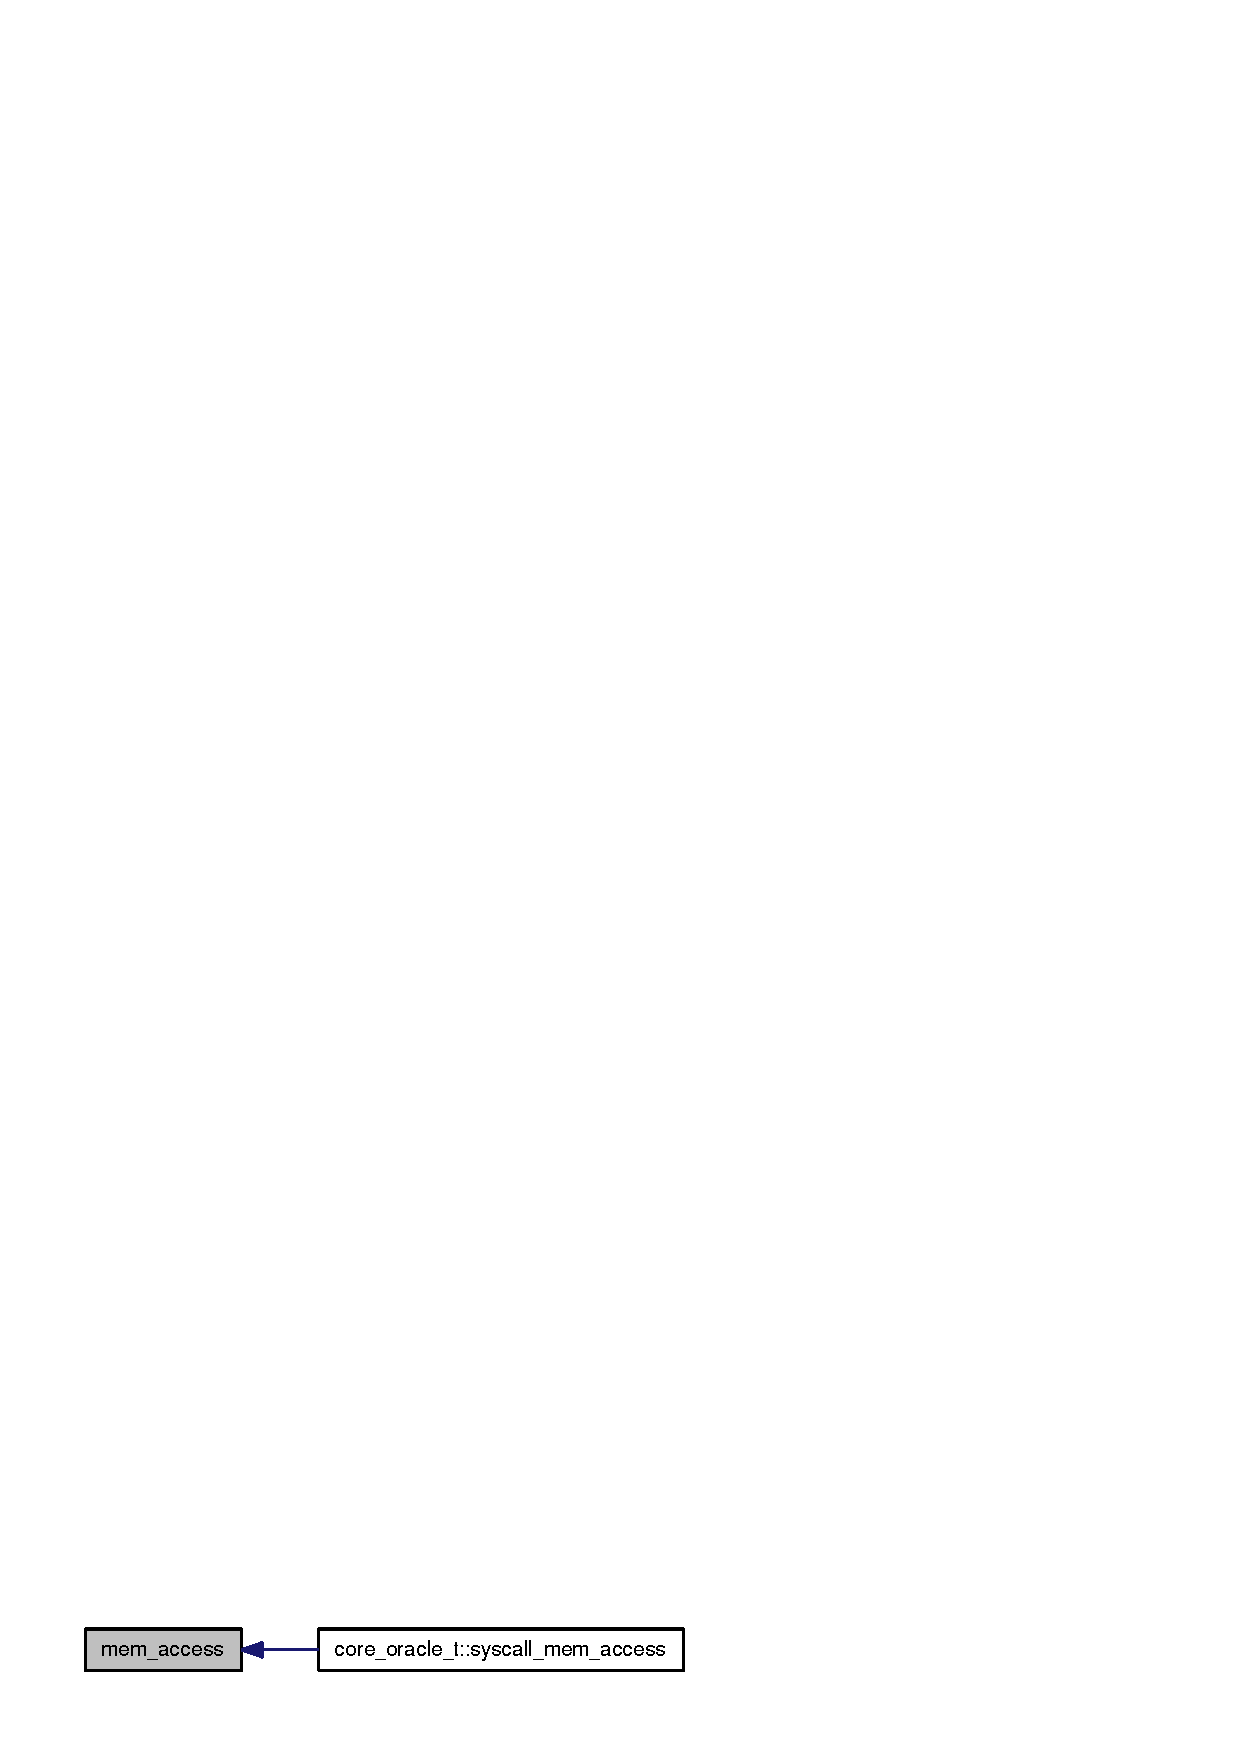
\includegraphics[width=166pt]{memory_8h_2b4368bb43fd552750bdf3f6e59b7c46_icgraph}
\end{center}
\end{figure}
\index{memory.h@{memory.h}!mem\_\-bcopy@{mem\_\-bcopy}}
\index{mem\_\-bcopy@{mem\_\-bcopy}!memory.h@{memory.h}}
\subsubsection[{mem\_\-bcopy}]{\setlength{\rightskip}{0pt plus 5cm}enum {\bf md\_\-fault\_\-type} mem\_\-bcopy (int {\em core\_\-id}, \/  {\bf mem\_\-access\_\-fn} {\em mem\_\-fn}, \/  struct {\bf mem\_\-t} $\ast$ {\em mem}, \/  enum {\bf mem\_\-cmd} {\em cmd}, \/  {\bf md\_\-addr\_\-t} {\em addr}, \/  void $\ast$ {\em vp}, \/  int {\em nbytes})}\label{memory_8h_9a8495a85883df0c1bef27d5acebad76}


\index{memory.h@{memory.h}!mem\_\-check\_\-fault@{mem\_\-check\_\-fault}}
\index{mem\_\-check\_\-fault@{mem\_\-check\_\-fault}!memory.h@{memory.h}}
\subsubsection[{mem\_\-check\_\-fault}]{\setlength{\rightskip}{0pt plus 5cm}enum {\bf md\_\-fault\_\-type} mem\_\-check\_\-fault (struct {\bf mem\_\-t} $\ast$ {\em mem}, \/  enum {\bf mem\_\-cmd} {\em cmd}, \/  {\bf md\_\-addr\_\-t} {\em addr}, \/  int {\em nbytes})}\label{memory_8h_369c3899ce6c337db4b74ddb1bdebc07}


\index{memory.h@{memory.h}!mem\_\-create@{mem\_\-create}}
\index{mem\_\-create@{mem\_\-create}!memory.h@{memory.h}}
\subsubsection[{mem\_\-create}]{\setlength{\rightskip}{0pt plus 5cm}struct {\bf mem\_\-t}$\ast$ mem\_\-create (char $\ast$ {\em name})\hspace{0.3cm}{\tt  [read]}}\label{memory_8h_5ef01d16da6ed478b982aec02df12ce1}


\index{memory.h@{memory.h}!mem\_\-delmap@{mem\_\-delmap}}
\index{mem\_\-delmap@{mem\_\-delmap}!memory.h@{memory.h}}
\subsubsection[{mem\_\-delmap}]{\setlength{\rightskip}{0pt plus 5cm}void mem\_\-delmap (struct {\bf mem\_\-t} $\ast$ {\em mem}, \/  {\bf md\_\-addr\_\-t} {\em addr}, \/  size\_\-t {\em length})}\label{memory_8h_e2a684d4da3b80d59c91949af34cb01c}


\index{memory.h@{memory.h}!mem\_\-init@{mem\_\-init}}
\index{mem\_\-init@{mem\_\-init}!memory.h@{memory.h}}
\subsubsection[{mem\_\-init}]{\setlength{\rightskip}{0pt plus 5cm}void mem\_\-init (struct {\bf mem\_\-t} $\ast$ {\em mem})}\label{memory_8h_63f8f683dd1f4b2489d34984bd3422df}


\index{memory.h@{memory.h}!mem\_\-newmap@{mem\_\-newmap}}
\index{mem\_\-newmap@{mem\_\-newmap}!memory.h@{memory.h}}
\subsubsection[{mem\_\-newmap}]{\setlength{\rightskip}{0pt plus 5cm}{\bf md\_\-addr\_\-t} mem\_\-newmap (struct {\bf mem\_\-t} $\ast$ {\em mem}, \/  {\bf md\_\-addr\_\-t} {\em addr}, \/  size\_\-t {\em length}, \/  int {\em mmap})}\label{memory_8h_2a66417821c1ecf1c49c05a5b4f37cf1}


\index{memory.h@{memory.h}!mem\_\-newmap2@{mem\_\-newmap2}}
\index{mem\_\-newmap2@{mem\_\-newmap2}!memory.h@{memory.h}}
\subsubsection[{mem\_\-newmap2}]{\setlength{\rightskip}{0pt plus 5cm}{\bf md\_\-addr\_\-t} mem\_\-newmap2 (struct {\bf mem\_\-t} $\ast$ {\em mem}, \/  {\bf md\_\-addr\_\-t} {\em addr}, \/  {\bf md\_\-addr\_\-t} {\em our\_\-addr}, \/  size\_\-t {\em length}, \/  int {\em mmap})}\label{memory_8h_15d8a89dbc649d4d22ede41ad760a4f4}


\index{memory.h@{memory.h}!mem\_\-newpage@{mem\_\-newpage}}
\index{mem\_\-newpage@{mem\_\-newpage}!memory.h@{memory.h}}
\subsubsection[{mem\_\-newpage}]{\setlength{\rightskip}{0pt plus 5cm}void mem\_\-newpage (struct {\bf mem\_\-t} $\ast$ {\em mem}, \/  {\bf md\_\-addr\_\-t} {\em addr})}\label{memory_8h_ad0101398be2daf0d519855f60504b7f}


\index{memory.h@{memory.h}!mem\_\-reg\_\-stats@{mem\_\-reg\_\-stats}}
\index{mem\_\-reg\_\-stats@{mem\_\-reg\_\-stats}!memory.h@{memory.h}}
\subsubsection[{mem\_\-reg\_\-stats}]{\setlength{\rightskip}{0pt plus 5cm}void mem\_\-reg\_\-stats (struct {\bf mem\_\-t} $\ast$ {\em mem}, \/  struct {\bf stat\_\-sdb\_\-t} $\ast$ {\em sdb})}\label{memory_8h_8707f3986260f7eb408598f1c8e4e5c5}


\index{memory.h@{memory.h}!mem\_\-strcpy@{mem\_\-strcpy}}
\index{mem\_\-strcpy@{mem\_\-strcpy}!memory.h@{memory.h}}
\subsubsection[{mem\_\-strcpy}]{\setlength{\rightskip}{0pt plus 5cm}enum {\bf md\_\-fault\_\-type} mem\_\-strcpy (int {\em core\_\-id}, \/  {\bf mem\_\-access\_\-fn} {\em mem\_\-fn}, \/  struct {\bf mem\_\-t} $\ast$ {\em mem}, \/  enum {\bf mem\_\-cmd} {\em cmd}, \/  {\bf md\_\-addr\_\-t} {\em addr}, \/  char $\ast$ {\em s})}\label{memory_8h_d4f0e69a043b9e0de5ba9b1237a2f645}


\index{memory.h@{memory.h}!mem\_\-translate@{mem\_\-translate}}
\index{mem\_\-translate@{mem\_\-translate}!memory.h@{memory.h}}
\subsubsection[{mem\_\-translate}]{\setlength{\rightskip}{0pt plus 5cm}{\bf byte\_\-t}$\ast$ mem\_\-translate (struct {\bf mem\_\-t} $\ast$ {\em mem}, \/  {\bf md\_\-addr\_\-t} {\em addr}, \/  int {\em dirty})}\label{memory_8h_17169f9bfb51490665d78c0ccc0b5023}


\index{memory.h@{memory.h}!page\_\-owner@{page\_\-owner}}
\index{page\_\-owner@{page\_\-owner}!memory.h@{memory.h}}
\subsubsection[{page\_\-owner}]{\setlength{\rightskip}{0pt plus 5cm}int page\_\-owner ({\bf md\_\-paddr\_\-t} {\em paddr})}\label{memory_8h_6d8733f7e3e27b600001064a1a8714c9}


\index{memory.h@{memory.h}!v2p\_\-translate@{v2p\_\-translate}}
\index{v2p\_\-translate@{v2p\_\-translate}!memory.h@{memory.h}}
\subsubsection[{v2p\_\-translate}]{\setlength{\rightskip}{0pt plus 5cm}{\bf md\_\-paddr\_\-t} v2p\_\-translate (int {\em core\_\-id}, \/  {\bf md\_\-addr\_\-t} {\em virt\_\-addr})}\label{memory_8h_5ce286b386b22428c54847fd33a31fb9}


\index{memory.h@{memory.h}!wipe\_\-memory@{wipe\_\-memory}}
\index{wipe\_\-memory@{wipe\_\-memory}!memory.h@{memory.h}}
\subsubsection[{wipe\_\-memory}]{\setlength{\rightskip}{0pt plus 5cm}void wipe\_\-memory (struct {\bf mem\_\-t} $\ast$ {\em mem})}\label{memory_8h_242fb835e054dfbb5a4a7e0d783ff72c}




\subsection{Variable Documentation}
\index{memory.h@{memory.h}!mem\_\-access\_\-fn@{mem\_\-access\_\-fn}}
\index{mem\_\-access\_\-fn@{mem\_\-access\_\-fn}!memory.h@{memory.h}}
\subsubsection[{mem\_\-access\_\-fn}]{\setlength{\rightskip}{0pt plus 5cm}enum {\bf md\_\-fault\_\-type}($\ast$ {\bf mem\_\-access\_\-fn})(int core\_\-id, struct {\bf mem\_\-t} $\ast$mem,enum {\bf mem\_\-cmd} cmd,{\bf md\_\-addr\_\-t} addr,void $\ast$p,int nbytes)}\label{memory_8h_b19d1d345069394f94dedcfe12c3d96a}


